\documentclass[UTF8, 12pt]{article}

% PACKAGES
\usepackage{geometry}
\usepackage{graphicx}
\usepackage{setspace}
\usepackage{indentfirst}
\usepackage{hyperref}
\usepackage{amsmath}
\usepackage[T1]{fontenc}
\usepackage[nottoc,notlot,notlof]{tocbibind}
\usepackage[style=ieee,sorting=anyt, backend=biber]{biblatex}

% DOCUMENT SETTINGS
% PAPER SETTINGS
\geometry{letterpaper,
          left=1in,
          right=1in,
          top=1in,
          bottom=1in}

% IMAGE DIRECTORY
\graphicspath{{images/}}

% OTHER SETTINGS
\renewcommand*\contentsname{Table of Contents} % change table of contents name
\renewcommand{\thefigure}{\Roman{figure}}
\addbibresource{refs.bib}

% TITLE DEFINITIONS
\title{Project Lab 2\\\large Midterm Report}
\author{Dirk Thieme\\R11636727\\Texas Tech University}
\date{October 2022}

% MAIN DOCUMENT
\begin{document}
\maketitle
\pagenumbering{gobble}
\newpage
\pagenumbering{arabic}
% \spacing{1.25}
\spacing{2}

% ABSTRACT
\begin{abstract}
    This paper describes the current progress of the Automated Recorder Project. While the requirements of the project will be discussed more in further sections, the general goal is to automate the playing of a recorder using a Raspberry Pi, which will be able to play any song as given to it through a flash drive. This project is being developed by Dirk Thieme, Mason Hadley, Jake Kiedasch, and Mariano Arce.
\end{abstract}

\newpage
\tableofcontents

\newpage
\listoffigures

% \newpage
% \listoftables

\newpage
\section{Introduction}
    The original premise of the Automated Recorder Project is to play a grade school recorder using a Raspberry Pi. The recorder should be able to play eight notes, and would be able to play a select number of songs chosen by the instructor of the course and a local area elementary school teacher. The recorder apparatus should be able to play in front of an elementary school class.

    While the premise of the project was enough of a challenge, this project aims to go above and beyond the original scope by allowing the recorder to play all 27 notes within its capability and by allowing the user to dynamically chose the desired song to play with an MP3 file. To allow the recorder to play all notes, certain holes must only be covered halfway, a technique known as leaking and pinching \cite{rec_wiki}. To be able to play any MP3 file provided, the software will be able to process the song on demand and convert the sound wave into a collection of frequencies which correspond to notes. These notes will be automatically converted into notes that the recorder can play.

    The brain of the apparatus is the Raspberry Pi 4B (furthermore Pi), a single-board computer which executes the code and controls the hardware. The Pi is powered using a quad core 64-bit ARM-Cortex A72 running at 1.5GHz \cite{ras_pi} which brings enough power to the table in order to complete the challenging digital signal processing required. The GPIO pins are also utilized to be able to control the hardware which actuates the recorder.

    The recorder is physically controlled through the use of six solenoids, three servo motors, and three compounded fans. Five of the solenoids cover and uncover the main holes, and three of the servos perform the pinching of the holes which require multiple positions. The one other solenoid opens and closes the main labium, which stops the recorder from playing to play rests. The solenoids require 12V power, while the servos and Pi require 5V power. The Pi only outputs 5V at 16mA on the GPIO pins \cite{ras_pi}, therefore a circuit has been designed in order to be able to actuate the solenoids while not burning out the GPIO pins. To power the entire setup, a 12V, 150W power supply will be able to accept AC wall power, which it can then send to a custom made power distribution PCB, which incorporates a 12V-5V buck converter and the various high power outputs, along with the solenoid circuits. 

    While the structure of the software is rather simple, the implementation is exceedingly complex, and requires immense amounts of research and assistance to complete. The software is not currently finalized, however in its current state it ingests an MP3 file then converts it into a WAV file. The WAV file bytestream is parsed into its proper values, then its time-domain signal is broken up into bins which are individually processed using a Fast Fourier Transform into their frequency-domain counterpart. The magnitudes of each bin are then calculated, which reveal the peak frequency of the bin, corresponding to the note at that time period. These notes are then converted into their recorder playable counterparts, which will then be played for the correct amount of time.

\newpage
\section{Body}
    The current state of this project is comprised of the following components, the Software, a Python codebase which consists of the MP3 ingestion, the WAV parsing, the Fast Fourier Transform, and the musical outputs, and the Hardware, which consists of the recorder itself, the control devices, the air production, and the Pi which runs the whole thing.

\subsection{Software}
\subsubsection{Flow of Control Chart}
    \begin{figure}[h]
        \centering
        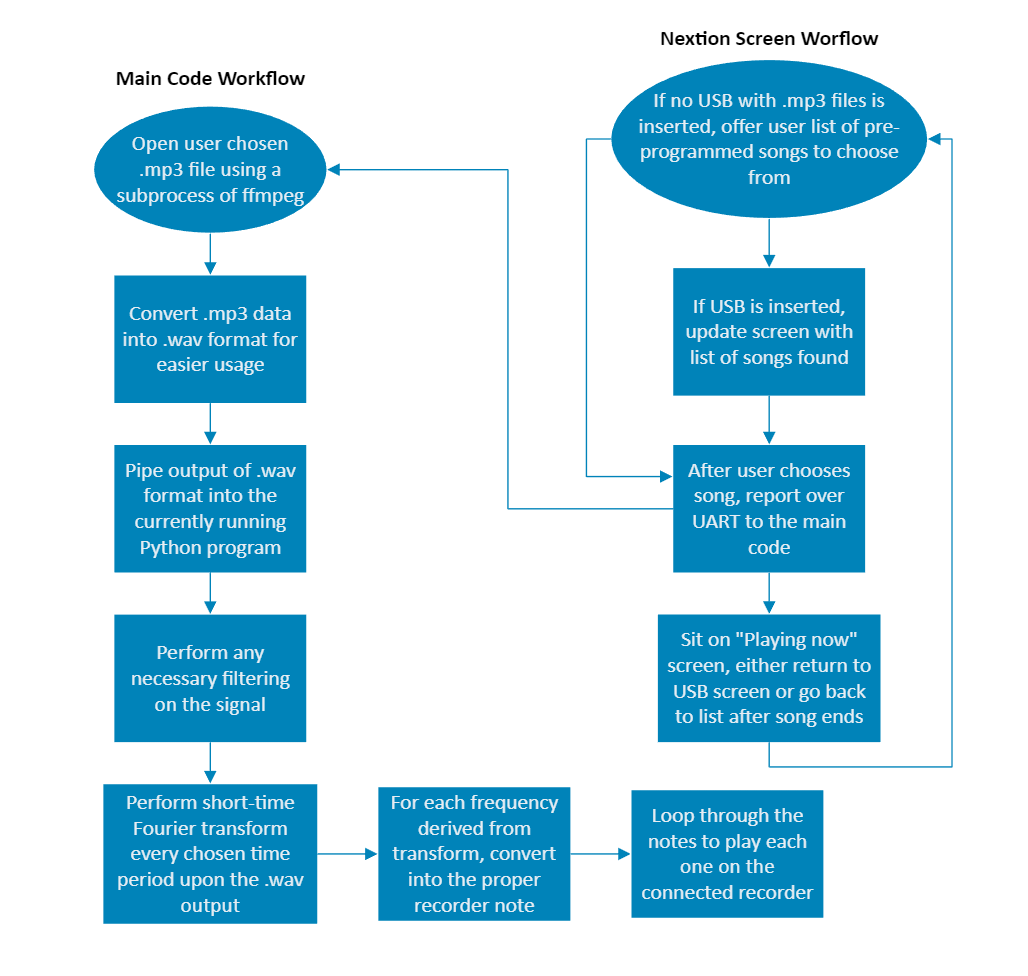
\includegraphics[width=0.75\textwidth]{flowchart}
        \caption{Main Software Flowchart}
        \label{fc}
    \end{figure}
    As shown in Figure \ref{fc}, this flowchart is the initial path which the code takes. The Nextion workflow has not yet been implemented, as it is unnecessary in determining if the main important code is functional, which itself cannot be yet determined without the construction of the apparatus. As stated previously, the code currently begins at the top if the "Main Code Workflow" section, however in the future it will begin at the "Nextion Screen Workflow". The Nextion screen is a touch screen with a built in microcontroller, which will be used to take user input and send it over to the Pi for actual use. 

\subsubsection{MP3 Ingestion}
    The bulk of the MP3 ingestion is performed by the software \textbf{ffmpeg}, originally developed by Fabrice Bellard and Bobby Bingham on December 20, 2000 \cite{ffmpeg}. 
    \begin{figure}[h]
        \centering
        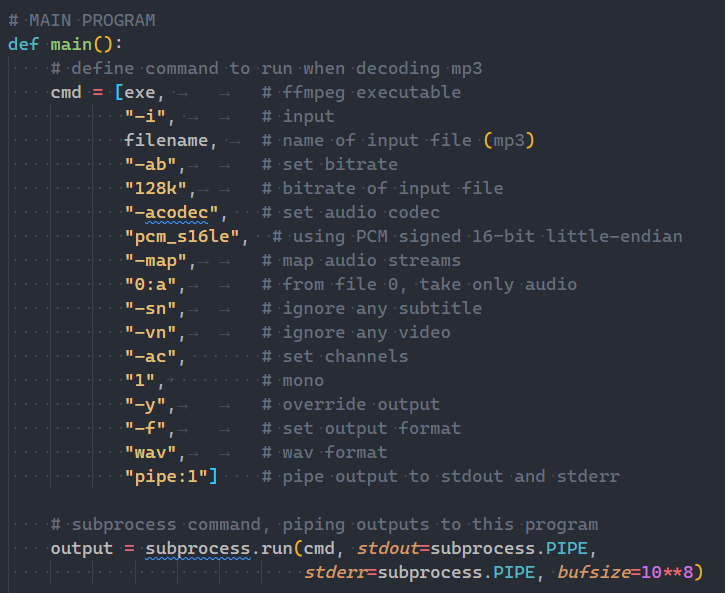
\includegraphics[width=0.75\textwidth]{ffmpeg_code}
        \caption{ffmpeg Command and Output Implementation}
        \label{ff_code}
    \end{figure}
    Shown in Figure \ref{ff_code}, certain command flags must be used upon executing the program in order to ensure proper output \cite{ffmpeg}. Some of the commands are less important, such as "-sn", which ignores subtitles or "-vn", which ignores any video streams (although this does implicate the software could feasibly process video data). Other commands are a necessity for proper output, such as "-f" and "wav", which sets the output format to a WAV file, and "-acodec" and "pcm\_s16le", which sets the output codec correctly. The most important flag there is "pipe:1" which outputs the WAV bytestream to the stdout, instead of dumping the output to a file. All of the output is contained in the variable conveniently named "output." Output consists of two properties, stderr and stdout. As stated above, stdout contains the bytestream of the output, but for debugging purposes stderr is useful as it contains the output of the command.

\subsubsection{WAV Parsing and Processing}
    Now that a WAV "file" has been obtained, work must be done in order to ascertain the correct values. The codec which was used to process the song is known as PCM, and the actual values that were output were unsigned 16-bit little-endian chunks. If one simply tried to read the bytes as they were, nothing but gibberish would be produced. This is because the bytes are little-endian, meaning the lower 8-bits are placed ahead of the upper 8-bits, effectively reversing the number in memory. As an example, take the decimal number \(2,500\). Its representation in a 16-bit hexadecimal is \(0x09C4\). Storing this value into contiguous memory locations would result in the following:
    \begin{equation*}
        0xC4 \to 0x09 \to ...
    \end{equation*}
    Attempting to get this value by only reading from left to right would return the number \(0xC409\), which is the decimal number \(50,185\), the incorrect value.

    To combat this, the Python package struct is used, as the programmer can tell the struct unpacking object what format to retrieve the bytestream as. This is done using format strings, in this case the string "<L". The < symbol tells the object the bytes will be little-endian, and the L tells the object to pack them into a 4-byte number \cite{struct}. This initial reading of the file allows the program to find the necessary sections of the file to read from.

    WAV files consist of a standardized structure \cite{wav}. They begin with a 44-76 byte header, depending on the WAV file creator. The program parses this header to either find the "fmt" section or the "data" section. The "fmt" section contains useful file information, such as number of channels, sample rate, and codec type. The "data" section contains, quite simply, all the actual song data. The program parses the "fmt" section for the information it needs to later process the "data" section. This is shown in below in Figure \ref{wav_code}.
    \begin{figure}[h!]
        \centering
        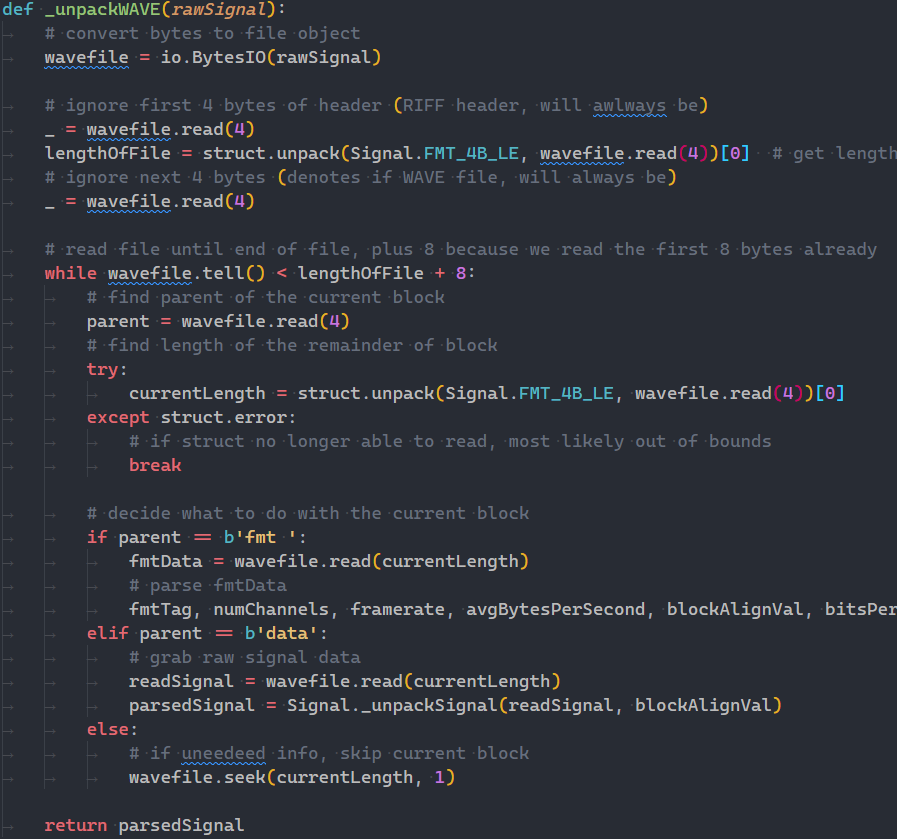
\includegraphics[width=0.55\textwidth]{wave_parse}
        \caption{WAV Processing Code}
        \label{wav_code}
    \end{figure}
    After this is complete, the variable "parsedSignal" is returned to the main program, which contains the actual waveform, and is then ready for further processing.

\subsubsection{The Fast Fourier Transform}
    While the program now has a long list of numbers which correspond to the waveform, shown below, the waveform itself is not a very useful signal for note processing.
    \begin{figure}[h]
        \centering
        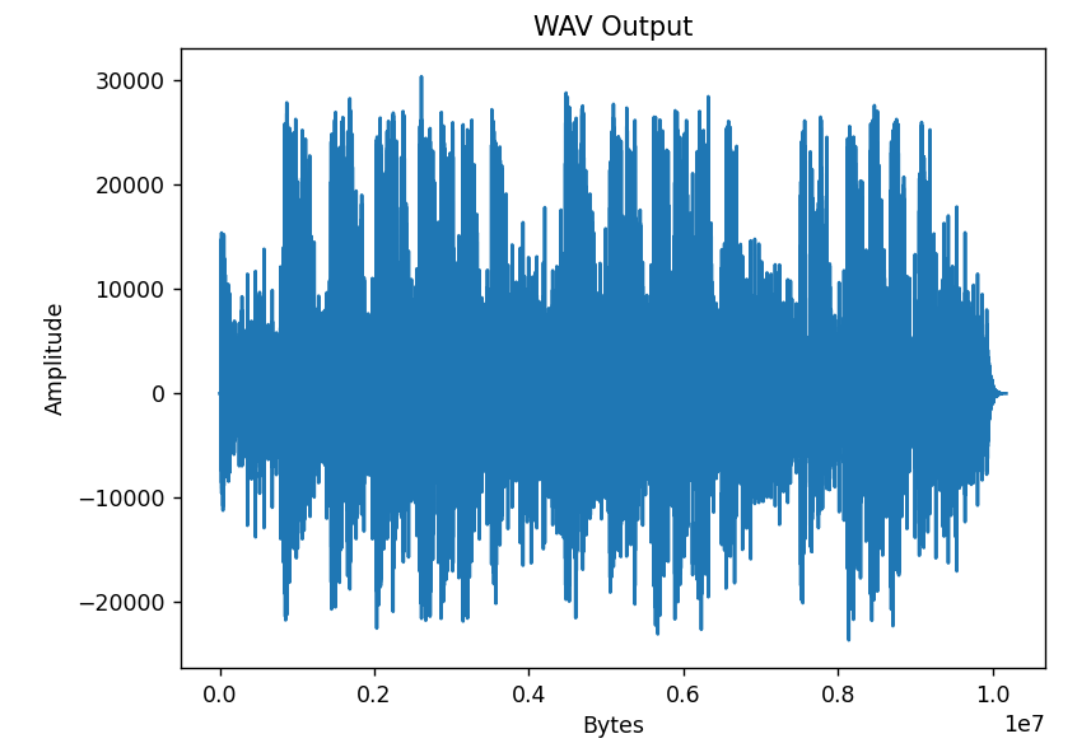
\includegraphics[width=0.75\textwidth]{waveform.png}
        \caption{An Example Waveform of a Song}
    \end{figure}
    These numbers are just the amplitude of the sound at that point in time, but to find the note at that point in time, the Fourier transform of the signal must be taken. The algorithm that has been implemented for live music processing is the Cooley-Tukey Fast Fourier Transform. This algorithm was popularized in 1965 by James Cooley of IBM and John Tukey of Princeton, although the original implementation was found to have been discovered in 1805 by Carl Friedrich Gauss \cite{fft_wiki}. The main premise is to recursively divide the Fourier transform into smaller and smaller chunks, which are then added back together at the end to produce the output \cite{fft_paper}. The standard Discrete Fourier Transform is defined by the equation \cite{fft_wiki}:
    \begin{equation}
        X_k = \sum_{n=0}^{N-1}x_ne^{-j2{\pi}kn/N} \quad k = 0 \; .. \; N - 1
    \end{equation}
    which is an $O(n^2)$ operation. The radix-2 algorithm brings this down to only $O(n\log{}n)$ through the recursion and division of the problem, leading to massive time and memory savings down the line.

    A prerequisite of this operation is that the provided signal must be a power of 2, which is where the time savings come from \cite{fft_wiki}. In order to this, the length of the signal is checked using the code in Figure \ref{check2_fig}, which compares the bits of the number and the number minus one. If the number is a power of 2, the result of ANDing them together would be 0, otherwise it would be any other number.
    \begin{figure}[h]
        \centering
        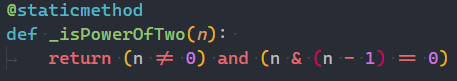
\includegraphics[width=0.75\textwidth]{check2.png}
        \caption{Function to Calculate if Number is a Power of 2}
        \label{check2_fig}
    \end{figure}
    Because the sample rate of the songs is 44.1kHz, and the windows of time are 100ms long, the number is not a power of 2, therefore the next highest power of 2 must be found and the signal must be extended to the new number.

    To find the next power of 2, a function which forces all the bits of the number to roll over until they are all 1's, then adds one to the number is used to calculate the next number to pad to. This is shown in Figure \ref{calc2_fig}.
    \begin{figure}[h!]
        \centering
        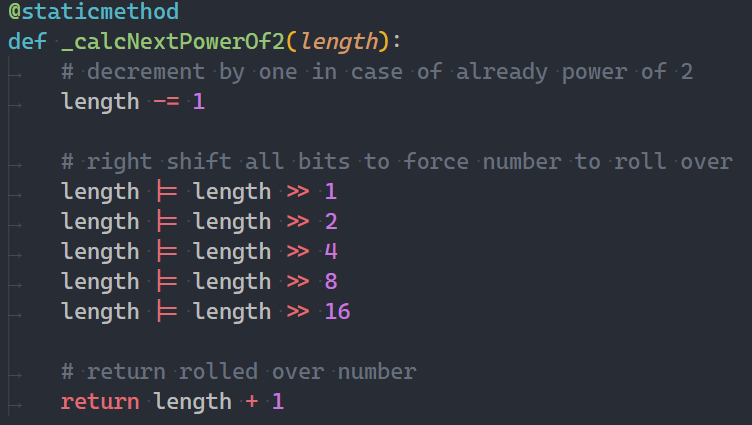
\includegraphics[width=0.7\textwidth]{calc2.png}
        \caption{Function to Find the Next Highest Power of Two}
        \label{calc2_fig}
    \end{figure}
    Once the signal is appropriately padded, the actual math can begin. The main algorithm consists of five steps:
    \newpage
    \begin{enumerate}
        \item Find the length of the current input list. If the length is one, return the list as is, otherwise continue.
        \item Using the length of the list, calculate $\omega$ using the formula $\omega = e^{j2\pi/N}$ where $N$ is the length.
        \item Break the current list into its odd and even elements.
        \item Pass the two new lists recursively into function.
        \item When the lists return, recombine the odd and even lists into a single list by raising $\omega$ to the current index of the loop and doing some other math.
    \end{enumerate}
    After these steps are completed the Fast Fourier Transform of the current list is complete.

\subsubsection{FFT Post-Processing}
    Once the waveform is converted from a time domain signal into a frequency domain signal, further work must be done to transform the current values into usable frequencies. To do this, the highest magnitudes of the bins of values must be calculated. To do this, simply take the real and imaginary 

\newpage
\printbibliography

\end{document}